%!TEX root = main.tex


\section{Probability with connectable submodels}

Throughout this paper, we will assume all measurable sets $X$ are finite sets. This is both because it makes explanations simpler and because it is easy to show that submodels exist in this setting (Lemma \ref{lem:subm_exist}). Many of the proofs in this paper can likely be specialised to more general settings due to our use of string diagrams which represent abstract morphisms in Markov categories, rather than finite Markov kernels specifically.

The standard method of constructing probability models introduces a probability space $(\prob{P},(\Omega,\sigalg{F}))$ with $\Omega$ a sample space, $\sigalg{F}$ a $\sigma$-algebra on $\Omega$ and $\prob{P}$ a probability measure on $(\Omega,\sigalg{F})$. Random variables are defined by measurable functions on $\Omega$ and are given names in sans-serif like $\RV{X}$. A probability distribution $\prob{P}^{\RV{XYZ}}$ is ``the joint distribution of $\RV{X}$, $\RV{Y}$ and $\RV{Z}$ under $\prob{P}$'' where $\RV{X},$ $\RV{Y}$ and $\RV{Z}$ are associated with random variables on $\Omega$ and is given by the pushforward of the function $\omega\mapsto (\RV{X}(\omega),\RV{Y}(\omega),\RV{Z}(\omega))$. Unless otherwise stated, a random variable named $\RV{X}$ will take values in the space $X$ (note the serif font).

To help us to construct causal models, we use an alternative method for building probability models. The motivation for doing this is to make it easy to represent a certain type of operation common in causal models. It is well-known that graphical causal models make use of operations that are not standard in probability theory. For example, in the causal graphical model framework, given $\prob{P}^{\RV{XYZ}}$, if $\RV{Z}$ blocks a backdoor path between $\RV{X}$ and $\RV{Y}$ then the backdoor adjustment formula allows us to define a new probability space with measure $\prob{P}_x$ via ``truncated factorisation'' \citep[page ~24]{pearl_causality:_2009}:

\begin{align}
	\prob{P}^{\RV{YZ}}_{x}(y,z):=\prob{P}^{\RV{Y|XZ}}(y|x,z)\prob{P}^{\RV{Z}}(z)\label{eq:truncated_fac}
\end{align}

The standard theory of probability does not assign special siginificance to the expression on the right side of Equation \ref{eq:truncated_fac}. At the same time, the notation we have chosen for the left side of Equation \ref{eq:truncated_fac} implicitly claims that $\prob{P}^{\RV{YZ}}_{x}$ is a distribution over the same variables $\RV{Y}$ and $\RV{Z}$ as the original $\prob{P}^{\RV{XYZ}}$. One way we can make sense of this is if $\prob{P}_{x}$ is defined on the same sample space as the original $\prob{P}$, and $\RV{Y}$ and $\RV{Z}$ are the same measurable functions on $\Omega$. However, in this case there is no guarantee that a suitable $\prob{P}_x$ exists. For example, if $\RV{X}=\RV{Z}$ (as in, $\RV{X}$ and $\RV{Z}$ are \emph{the same function on }$\Omega$) then there will usually be no measure $\prob{P}_x$ such that $\prob{P}^{\RV{YZ}}_{x}(y,z)$ agrees with Equation \ref{eq:truncated_fac} for any $\RV{Y}$ or $\prob{P}$.

A similar question arises in the framework of structural causal models. Such models posit a collection of \emph{structural equations}:
\begin{align}
	\RV{X}=f(\xi)\\
	\RV{Y}=g(\RV{X},\xi)
\end{align}
along with an operation of \emph{intervention} that can replace the right hand side of each equation. One can ask: are structural equations definitions of the random variables $\RV{X}$ and $\RV{Y}$, in which case intervention is an operation that apparently changes their definition, or are they instead statements of equalities that happen to hold with probability 1? The latter might seem to fit better with the view that these equations can be replaced, but there are at least some cases in which some variables \emph{are} defined to be equal to functions of other variables. For example (recalling our discussion in the introduction), any variable $\RV{B}$ representing a person's body mass index should surely be equal \emph{by definition} to $\frac{\RV{W}}{\RV{H}^2}$ where $\RV{W}$ represents their weight in kilograms and $\RV{H}$ represents their height in metres. 

One way to approach this is to note that there are two notions of equality of random variables - they can be strictly equal as functions on $\Omega$, and they can be almost surely equal with respect to some probability $\prob{P}$. Perhaps structural equations are statements of equality of the latter type. However, a statement of almost sure equality does not rule out strict equality -- in fact, it is necessary that almost sure equality holds for strict equality to hold. Furthermore, strict equalities have an impact on which interventions are possible (see body mass index above). Thus it seems that to fully specify a structural causal model we need to explicitly define the sample space and random variables in addition to the structural equations. But doing so is a hassle that, just like everyone else who works with probability theory, we would prefer to avoid.

While Potential Outcomes, which features no ``intervention'' operation, does not seem to raise the particular questions discussed above, we still find our approach useful for discussing questions like how ``consequences of actions'' relate to ``potential outcomes'', as discussed in the introduction.

The fundamental idea behind our approach is to define variables as ``names'' along with sets of possible values. We suggest that variable names can act as indicators of ``what the variable is modelling''. We think advantages of this approach is, essentially, that we can choose how much structure we want to give variable names:
\begin{itemize}
	\item We do not need to fully specify a sample space and a set of functions to define variables
	\itme We do not need to specify a default sample space and set of functions that might rule out interventions (e.g. if structural equations are variable definitions) or rule out the possibility that body mass index $\RV{B}$ and $\frac{\RV{W}}{\RV{H}^2}$ are the same thing (e.g. if every symbol is associated 1:1 with a projection from some big Cartesian product)
\end{itemize}

\subsection{Markov categories}
Before we introduce our definition of variables, we will briefly introduce the theory of \emph{Markov categories}, which we will build our approach on top of.

We are working with a ``probability theory'' constructed with finite sets and Markov kernels that map from one set to probability distributions on another. The category with finite sets as objects and Markov kernels as morphisms along with some additional elements we will introduce shortly is known to be an example of a Markov category \citep{fritz_synthetic_2020}. In the words of Fritz, if one wants to model flow of information, the model one adopts will generally satisfy the requirements of Markov categories. In particular, all formalisations of probability theory satisfy the requirements of Markov categories, including the formalisation we work with here consisting of finite sets and Markov kernels.

The string diagram notation we introduce is an abstract notation for reasoning in Markov categories; a valid derivation in a string diagram corresponds to a valid proof in any Markov category. This is complicated by the fact that while we use standard notation for the ``pictorial'' aspects of these diagrams, we also annotate wires with variable names as an extension of this notation. 

\todo[inline]{I don't really know where that leaves me overall}

The basics of the graphical notation are as follows: a Markov kernel is represented as a box and a probability distribution as a triangle:

\begin{align}
\kernel{K}&:=\begin{tikzpicture}[baseline={([yshift=-.5ex]current bounding box.center)}]
	\path (0,0) node (A) {}
	++ (0.5,0) node[kernel] (K) {$\kernel{K}$}
	++ (0.5,0) node (B) {};
	\draw (A) -- (K) -- (B);
\end{tikzpicture}\\
\prob{P}&:= \begin{tikzpicture}[baseline={([yshift=-.5ex]current bounding box.center)}]
	\path (0,0) node[dist] (K) {$\kernel{K}$}
	++ (0.5,0) node (B) {};
	\draw (K) -- (B);
\end{tikzpicture}
\end{align}

Two Markov kernels $\kernel{L}:X\to \Delta(Y)$ and $\kernel{M}:Y\to \Delta(Z)$ have a product $\kernel{L}\kernel{M}:X\to \Delta(Z)$ given by the matrix product: $\kernel{L}\kernel{M}_x^z = \sum_y \kernel{L}_x^y\kernel{M}_y^z$. Graphically, we write represent products by joining kernel wires together:

\begin{align}
	\kernel{L}\kernel{M}:= \begin{tikzpicture}[baseline={([yshift=-.5ex]current bounding box.center)}]
	\path (0,0) node (A) {}
	++ (0.5,0) node[kernel] (K) {$\kernel{K}$}
	++ (0.7,0) node[kernel] (M) {$\kernel{M}$}
	++ (0.5,0) node (B) {};
	\draw (A) -- (K) -- (M) -- (B);
\end{tikzpicture}
\end{align}

The Cartesian product $X\times Y:=\{(x,y)|x\in X, y\in Y\}$.

Given kernels $\kernel{K}:W\to Y$ and $\kernel{L}:X\to Z$, the tensor product $\kernel{K}\otimes\kernel{L}:W\times X\to \Delta(Y\times Z)$ is defined by $(\kernel{K}\otimes\kernel{L})_{(w,x)}^{(y,z)}:=K_{w}^y L_{x}^z$.

The tensor product is represeted by parallel juxtaposition:

\begin{align}
	\kernel{K}\otimes \kernel{L}&:=\begin{tikzpicture}[baseline={([yshift=-.5ex]current bounding box.center)}]
	\path (0,0) node (A) {$W$}
	++ (0.5,0) node[kernel] (K) {$\kernel{K}$}
	++ (0.5,0) node (B) {$Y$};
	\path (0,-0.5) node (C) {$X$}
	++ (0.5,0) node[kernel] (L) {$\kernel{L}$}
	++ (0.5,0) node (D) {$Z$};
	\draw (A) -- (K) -- (B);
	\draw (C) -- (L) -- (D);
\end{tikzpicture}
\end{align}

We read diagrams from left to right (this is somewhat different to \citet{fritz_synthetic_2020,cho_disintegration_2019,fong_causal_2013} but in line with \citet{selinger_survey_2010}). They are to be read as a series of products of Markov kernels. For some special Markov kernels, we can replace the generic ``box'' of a Markov kernel with a special diagrammatic element that is visually suggestive of what they accomplish.

Markov categories feature a number of Markov kernels that play special roles in the theory. They are defined abstractly in Appendix \ref{sec:app_mcat}. Their visual representation is as follows:

The identity map is a bare line:

\begin{align}
	\mathrm{Id}_X&:=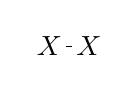
\begin{tikzpicture}[baseline={([yshift=-.5ex]current bounding box.center)}]
	\path (0,0) node (A) {$X$} ++ (0.5,0) node (B) {$X$};
	\draw (A) -- (B);
\end{tikzpicture}
\end{align}

The erase map is a fuse:

\begin{align}
	\text{del}_X&:=\begin{tikzpicture}[baseline={([yshift=-.5ex]current bounding box.center)}]
	\path (0,0) ++ (1,0) node (B) {$X$};
	\draw[-{Rays[n=8]}] (A) -- (B);
\end{tikzpicture}
\end{align}

The copy map is a fork:

\begin{align}
	\text{copy}_X&:=\begin{tikzpicture}[baseline={([yshift=-.5ex]current bounding box.center)}]
	\path (0,0) node (A) {$X$} 
	++ (0.5,0) node[copymap] (copy0) {}
	++ (0.5,0.15) node (B) {$X$}
	+ (0,-0.3) node (C) {$X$};
	\draw (A) -- (copy0) to [out=45,in=180] (B) (copy0) to [out=-45, in=180] (C);
\end{tikzpicture}
\end{align}

The swap map swaps wires:

\begin{align}
	\text{swap}_X &:=  
\begin{tikzpicture}[baseline={([yshift=-.5ex]current bounding box.center)}]
		\path (0,0) node (A) {} 
		+ (0,-0.5) node (B) {}
		++ (1,0) node (C) {}
		+ (0,-0.5) node (D) {};
		\draw (A) to [out=0,in=180] (D) (B) to [out=0, in=180] (C);
	\end{tikzpicture}
\end{align}

Because we anticipate that the graphical notation will be unfamiliar  to maney, we will also include translations to more familiar notation.

\subsection{Finite set probability theory}

For our purposes, a Markov kernel $\kernel{K}:X\to \Delta(Y)$ is a map from $X$ to probability distributions on $Y$. We can represent it concretely by the elements $(\kernel{K}_{x}^y)_{x\in X, y\in Y}$. An element $K_x^y$ represents the probability of $y\in Y$ given the argument $x\in X$. In general, an argument $w$ appearing as a superscript can be read as ``the probability of $w$'' and an argument $v$ appearing as a subscript can be read as ``given $v$''. Note that we do \emph{not} use Einstein summation in any expressions in this paper -- all sums will be written out explicitly.

A Markov kernel must have the following properties:
\begin{align}
	0\leq &K_{x}^y \leq 1 &\forall x,y\\
	\sum_{y\in Y} K_{x}^y &= 1 & \forall x
\end{align}

A probability distribution is a Markov kernel $\kernel{P}:\{*\}\to \Delta(Y)$ where $\{*\}$ is a one-element set. Such a Markov kernel can be represented as a matrix with one row, i.e. a column vector.

The erase map $\text{del}_X:X\to \{*\}$ is represented by the matrix $(\text{del}_X)_x = 1$ for all $x\in X$. It maps every element of $X$ to the unique probability distribution on $\{*\}$, which gives probability 1 to $*$, the only element of the set; we can think of this as forgetting the input.

The copy map $\text{copy}_X: X\to \Delta(X\times X)$ is the Markov kernel represented by the matrix $(\text{copy}_X)_x^{x',x''}:= \llbracket x = x' \rrbracket \llbracket x=x''\rrbracket$, where the iverson bracket $\llbracket \cdot \rrbracket$ evaluates to $1$ if $\cdot$ is true and $0$ otherwise. We can think of the copy map as taking an element $x$ and outputting a joint distribution of two ``variables'' that are deterministically equal to $x$.

A swap map $\text{swap}_X: X\times Y \to \Delta(Y\times X)$ is the Markov kernel represented by the matrix $(\text{swap}_X)_{x,y}^{y',x'}:=\llbracket x=x' \rrbracket \llbracket y=y'\rrbracket$. It takes two inputs and returns a joint distribution on two ``variables'' deterministically equal to the swapped inputs.

\subsection{Revisiting truncated factorisation}

Recall the problem of using non-standard operations like Equation \ref{eq:truncated_fac}, and our concerns regarding the fact that such operations might conflict with random variable definitions. Abstract Markov categories allow us to consider similar operations with no apparent concerns. Note that $P^{\RV{Y|XZ}}$ must be represented by a Markov kernel $\kernel{K}:X\times Z\to \Delta(Y)$ and $\prob{P}^{\RV{Z}}$ by a Markov kernel $\kernel{L}\in \Delta(Z)$ (we will explain later why we explicitly distinguish Markov kernels from conditional probabilities). Then we can define a Markov kernel $\kernel{M}:X\to \Delta(X\times Z)$ representing $x\mapsto \prob{P}^{\RV{YZ}}_{x}(y,z)$ by

\begin{align}
	\kernel{M}:= \tikzfig{truncated_factorisation}\label{eq:tfac_setted}
\end{align}

This is possible whenever $\kernel{K}$ and $\kernel{L}$ have the appropriate signatures, which seems to get around the issues regarding random variable definitions. However, we have accomplished this by substituting \emph{variables} for \emph{sets}, and sets are not an adequate substitute for variables. Consider an arbitrary Markov kernel $\kernel{K}:\{*\}\to \Delta(X\times X)$. We could draw this:
\begin{align}
	\kernel{K}:= \tikzfig{double_label}\label{eq:double_label}
\end{align}
In particular, we label both wires with $X$. However, it would be inappropriate to interpret this label as referring to a variable. Any Markov kernel representing ``the probability of $(\RV{X},\RV{X})$'' must surely require both copies of $\RV{X}$ to be deterministically equal. However, the relationship between the two in Equation \ref{eq:double_label} can be arbitrary.

Our solution to this is to distinguish \emph{names}, \emph{sets of values} and \emph{variables}. A name is, broadly speaking, a unique identifier and a variable is a name together with a set of values. If we say a variable $\RV{X}$ stands for a question like ``Will this coin come up heads?'', we could choose the name to correspond to the English sentence ``Will this coin come up heads?''. Formally this only means that there is no other variable that also has this name, but it also does the job of communicating informally what we intend this variable to represent. Names do not have to be of this form; for example, I could choose all my names to be functions on a common sample space $\Omega$ and perhaps offer a natural language explanation of what that sample space represents. However, for our purposes a variable is a unique identifier along with a set of values.

The unique identifier is introduced to addresses the problem described above: it's fine for two different variables to take values in the same set, and we generally do not require them to always take the same value. However, two instances of the same variable should always take the same value.

We define a variable as a Cartesian product $A\times B$ where $A$ is the single-element set containing the variable name and $B$ is the set of values it can take. Thus a variable is a set of (name, value) pairs such ats $\{(\RV{X},a),(\RV{X},b)\}$.

We require the following to be true of variables:

\begin{enumerate}
	\item \textbf{Uniqueness:} Given resolution sets $A\times X$ and $B\times Y$, if $A=B$ then $X=Y$
\end{enumerate}

We use sans serif letters $\RV{X},\RV{Y}$ to refer to names of variables and, due to the uniqueness axiom, also to variables. Given a variable $\RV{X}=A\times X$ we say ``$\RV{X}$ takes values in $X$''.


We define the product and projection of variables as follows:

\begin{itemize}
	\item \textbf{Product:} Given variables $\RV{W}=A\times X$ and $\RV{V}=B\times Y$, the product $\RV{W}\otimes\RV{V}=(A\times B)\times (X\times Y)$
	\item \textbf{Projection:} The projection $\pi_i$ is defined by $\pi_j:\bigotimes_{i\in I} \RV{X}_i = \RV{X}_j$
\end{itemize}

\todo[inline]{Show that these induce a symmetric monoidal category. One thing we need is that $A\times B$ is not isomorphic to $B$, and I'm not sure how to say this exactly.}

% In the category of sets, $(A\times B)\times (X\times Y)$ is naturally isomorphic to $\RV{W}\times\RV{V}=(A\times X)\times(B\times Y)$, and thus $\pi_i$ is naturally isomorphic to the canonical projection $\nu_j:\bigtimes_{i\in I} A_i = A_j$.

Define the variable $*:=\{\emptyset\}\times\{\emptyset\}$.

\begin{lemma}[Identity element]\label{lem:se_id}
For all variables $\RV{X}$, $\RV{X}\otimes * \cong *\otimes \RV{X} \cong \RV{X}$
\end{lemma}

\begin{proof}
Let $\RV{X}=A\times B$.
\begin{align}
	*\otimes \RV{X} &= (\{\emptyset\}\times A)\times(\{\emptyset\}\times B)\\
					&\cong A\times B\\
					&\cong (A\times \{\emptyset\})\times(B\times \{\emptyset\})\\
					&= \RV{X}\otimes *
\end{align}
\end{proof}

The following lemma guarantees that if we can divide a sequence $\RV{Z}$ into some collection of subsequences $\{\RV{A}_i\}_{i\in [n]}$, then we can find a collection of labeled sets corresponding to each subsequence $\RV{A}_i$.

Rather than using the $\otimes$ symbol to refer to the product of variables, which is somewhat overloaded, we will use the more familiar notation $(\RV{X},\RV{Y})$. Note that $(\{\RV{X}\}\times A)\otimes (\{\RV{Y}\}\times B) = \{(\RV{X},\RV{Y})\}\times (A\times B)$, so the notation $(\RV{X},\RV{Y})$ is the name of the variable obtained from taking the product of the two associated resolution sets.

\subsection{Markov variable maps}\label{sec:labeled_kernels}

We will call the morphisms of our category of variables \emph{Markov variable maps}. A Markov variable map $\model{K}:\RV{A}\to \Delta(\RV{B})$ is defined by a triple $(\kernel{K}^U,\RV{A},\RV{B})$, and can be thought of as a Markov kernel that maps between variables rather than between sets of values. If $\RV{A}$ takes values in $X$ and $\RV{B}$ takes values in $Y$, we define $\kernel{K}$ as follows for all $x\in X$, $y\in Y$:

\begin{align}
	\kernel{K}_{\RV{A},x}^{\RV{B},y}  = \kernel{K}^{U y}_x
\end{align}

We call $\kernel{K}^U:X\to \Delta(Y)$ the \emph{underlying Markov kernel}.

Suppose we have Markov variable maps $\kernel{K}:\RV{A}\to \Delta(\RV{B})$ and $\kernel{L}:\RV{C}\to \Delta(\RV{D})$. Then $\kernel{K}=\kernel{L}$ iff $\RV{A}= \RV{C}$ and $\RV{B}= \RV{D}$ and $\kernel{K}^U=\kernel{L}^U$.

Given $\kernel{K}:\RV{A}\to \Delta(\RV{B})$ and $\kernel{L}:\RV{B}\to \Delta(\RV{C})$, the product $\kernel{K}\kernel{L}$ is given by

\begin{align}
	\kernel{K}\kernel{L} = (\kernel{K}^U\kernel{L}^U,\RV{A},\RV{C})
\end{align}

Note that we don't allow products of Markov variable maps if they have compatible value sets but different variables. Going back to our example of viewing variables as questions, this can be thought of as disallowing the product of a variable map that answers the question ``will this coin land heads?'' with a variable map that depends on the answer to the question ``am I taller than my brother?''.

The diagrams representing Markov variable maps are identical to the diagrams representing their underlying Markov kernels decorated with variable names on each input and each output wire. 

A variable name could be a sequence of other variable names $(\RV{X}_i)_{i\in [n]}$. By construction, this means that we have a collection of variables $\RV{X}_i$ such that $(\RV{X}_i)_{i\in [n]}$ is the variable name associated with the product $\bigotimes_{i\in [n]} \RV{X}_i$. If each $\RV{X}_i$ takes values in a set $X_i$, then $(\RV{X}_i)_{i\in [n]}$ must take values in $\bigtimes_{i\in [n]} X_i$. The underlying Markov kernel can always be drawn with one wire representing each $X_i$, and using such a representation it is possible to assign each $\RV{X}_i$ in the sequence to a corresponding wire.

For example, if $\kernel{K}:(\RV{A}_1,\RV{A}_2)\to \Delta(\RV{B}_1,\RV{B}_2)$, for example, we can draw:

\begin{align}
	\kernel{K} := \begin{tikzpicture}[baseline={([yshift=-.5ex]current bounding box.center)}]
	\path (0,0) node (A1) {$\RV{A}_1$}
	+ (0,-0.3) node (A2) {$\RV{A}_2$}
	++ (0.7,-0.15) node[kernel] (K) {$\kernel{K}$}
	++ (0.7,0.15) node (B1) {$\RV{B}_1$}
	+ (0,-0.3) node (B2) {$\RV{B}_2$};
	\draw (A1) -- ($(K.west) + (0,0.15)$) (A2) -- ($(K.west) + (0,-0.15)$);
	\draw (B1) -- ($(K.east) + (0,0.15)$) (B2) -- ($(K.east) + (0,-0.15)$);
\end{tikzpicture}
\end{align}

or

\begin{align}
	\kernel{K} = \begin{tikzpicture}[baseline={([yshift=-.5ex]current bounding box.center)}]
	\path (0,0) node (A1) {$(\RV{A}_1,\RV{A}_2)$}
	++ (1.3,0) node[kernel] (K) {$\kernel{K}[\model{L}]$}
	++ (1.3,0.) node (B1) {$(\RV{B}_1,\RV{B}_2)$};
	\draw (A1) -- (K) -- (B1);
\end{tikzpicture}
\end{align}

A Markov variable maps must satisfy the following axiom.

\begin{enumerate}
	\item \textbf{Deterministic equality of identical variables:} For any Markov variable map $\kernel{K}:\RV{A}\to \Delta(\RV{B})$, the same variable may be assigned to two terminal wires in a graphical representation if there is a valid graphical representation of $\kernel{K}$ in which those two terminals are connected by a path and that path is not obstructed by any boxes or triangles.
\end{enumerate}

\begin{lemma}[Deterministic equality of identical variables]
This axiom is equivalent to the following three conditions:

Given $\kernel{K}:(\RV{X},\RV{Y})\to \Delta(\RV{X},\RV{Z})$, there exists some $\kernel{H}:X\times Z\to \Delta(Y)$ such that
\begin{align}
	\kernel{K} &= \begin{tikzpicture}[baseline={([yshift=-.5ex]current bounding box.center)}]
					\path (0,0) node (X) {$\RV{X}$}
					+ (0,-0.65) node (Z) {$\RV{Z}$}
					++ (0.5,0) node[copymap] (copy0) {}
					++ (0.7,-0.5) node[kernel] (L) {$\kernel{H}$}
					++ (0.9,0.65) node (Xout) {$\RV{X}$}
					+  (0,-0.65) node (Y) {$\RV{Y}$};
					\draw (X) -- (copy0) to [out=-45,in=180] ($(L.west) + (0,0.15)$) (L) -- (Y);
					\draw (copy0) to [out=45,in=180] (Xout);
					\draw (Z) -- ($(L.west) + (0,-0.15)$);
				 \end{tikzpicture}\label{eq:extn1}\\
	 	&\iff\\
	 \kernel{K}_{xz}^{x'y} &= \llbracket x=x'\rrbracket \kernel{H}_{xz}^{y}
\end{align}

Given $\kernel{L}: \RV{Z}\to \Delta(\RV{X},\RV{X},\RV{Y})$, we require that there exist some $\kernel{G}:\RV{Z}\to \Delta(\RV{X}, \RV{Y})$ such that
\begin{align}
	\kernel{L} &= \begin{tikzpicture}[baseline={([yshift=-.5ex]current bounding box.center)}]
					\path (0,0) node (Z) {$\RV{Z}$}
					++ (0.9,0) node[kernel] (L) {$\kernel{G}$}
					++ (0.9,0.15) node[copymap] (copy0) {}
					++ (0.5,0.3) node (X1) {$\RV{X}$}
					++ (0,-0.3) node (X2) {$\RV{X}$}
					++  (0,-0.3) node (Y) {$\RV{Y}$};
					\draw ($(L.east) + (0,0.15)$) -- (copy0) to[out=0,in=180] (X2);
					\draw (copy0) to [out=45,in=180] (X1);
					\draw (Z)--(L) ($(L.east) + (0,-0.15)$) -- (Y);
				 \end{tikzpicture}\label{eq:extn2}\\
			   &\iff\\
		\kernel{L}_{z}^{xx'y} &= \llbracket x=x' \rrbracket\kernel{G}_{z}^{xy}	   
\end{align}

There is no $\kernel{M}:(\RV{X},\RV{X},\RV{Y})\to \Delta(\RV{W},\RV{Z})$.
\end{lemma}

\begin{proof}
Suppose some variable $\RV{X}$ appears 
\end{proof}

\todo[inline]{If the category of variables and Markov variable maps is symmetric monoidal..}

There is a natural isomorphism between two Markov variable maps  $\kernel{K}$ and $\kernel{L}$ if one can be obtained from the other by application of a sequence of swaps. For example, if we have $\kernel{K}:(\RV{X},\RV{Y})\to \Delta(\RV{Z},\RV{W})$ and $\kernel{L}:(\RV{Y},\RV{X})\to \Delta(\RV{W},\RV{Z})$, then $\kernel{K}\cong \kernel{L}$ if

\begin{align}
\tikzfig{equivalence}
\end{align}

\subsection{Connection}

Connection is an associative operation $\rightrightarrows$ that ``joins'' two labeled Markov kernels where the labels can be matched and preserves unmatched inputs and outputs. A key property of connection is that, if both input Markov kernels satisfy Axiom 1, then the output also satisfies axiom 1. One can think of this operation like connecting two lego bricks of different sizes -- we connect all the parts that will fit together, and all the connection points that don't fit are left available.

For some variable $\RV{W}$, we use $m_{\RV{W}}(\RV{X})$ to refer to the number of times $\RV{W}$ appears in $\RV{X}$ (recalling that $\RV{X}$ may be a sequence of other variables). We say $\RV{W}$ is in $\RV{X}$ or $\RV{W}\in \RV{X}$ if $m_{\RV{W}}(\RV{X})>0$.

With this in mind, we define the following operations on sequences of labels

\begin{enumerate}
	\item \textbf{Difference of label sequences:} Given $\RV{X}_1$, $\RV{X}_2$, the difference $\RV{X}_1\setminus \RV{X}_2$ is a variable $\RV{X}_3$ such that for all variables $\RV{W}_i$, $m_{\RV{W}_i}(\RV{X}_3) = \max(0,m_{\RV{W}_i}(\RV{X}_1)-m_{\RV{W}_i}(\RV{X}_2))$
	\item \textbf{Intersection of labels:} Given $\RV{X}_1$, $\RV{X}_2$, the intersection $\RV{X}_1\cap \RV{X}_2$ is a variable $\RV{X}_3$ such that for any variable $\RV{W}_i$, $m_{\RV{W}_i}(\RV{X}_3) = \min(m_{\RV{W}_i}(\RV{X}_1),m_{\RV{W}_i}(\RV{Y}_2))$
\end{enumerate}

These definitions are non-unique in that they do not define the order of the resulting label sequence. This doesn't cause a problem because we only care about Markov variable maps that are identical up to isomorphism.

Given two Markov variable maps $\kernel{F}:\RV{I}_F\to\Delta(\RV{O}_F)$ and $\kernel{S}:\RV{I}_S\to\Delta(\RV{O}_S)$, make the following variable identifications:
\begin{align}
	\RV{O}_{F\cdot}&:=\RV{O}_F\setminus\RV{I}_S &\text{Variables only in the output of } \kernel{F}\\
	\RV{O}_{FS}&:=\RV{O}_F\cap\RV{I}_S &\text{Variables in the output of both}\\
	\RV{I}_{F\cdot} &:= \RV{I}_F\setminus \RV{I}_S &\text{Variables only in the input } \kernel{F}\\
	\RV{I}_{FS}&:= \RV{I}_F\cap\RV{I}_S &\text{Variables in the input of both}\\
	\RV{I}_{\cdot S}&:= \RV{I}_S\setminus \RV{I}_F &\text{Variables only in the input of }\kernel{S} \\
	\RV{O}_{I_FO_S*}&:=\RV{O}_S\cap \RV{I}_F\setminus \RV{I}_S &\text{Input of }\kernel{F}\text{ and the output only of }\kernel{S}\\
	\RV{O}_{O_FO_S*} &:= \RV{O}_F\cap\RV{O}_S\setminus \RV{I}_S&\text{Output of }\kernel{F}\text{ and the output only of }\kernel{S}\\
\end{align}

$\kernel{F}$ can be connected to $\kernel{S}$ iff $\RV{O}_{I_FO_S*}$ synonymous with $*$ and $\RV{O}_{O_FO_S*}$ is also synonymous with $*$. The reason for this is that, in general, if these sets were non-empty then we would not have a way to connect $\kernel{F}$ and $\kernel{S}$ without violating the deterministic equality of identical variables.

\begin{definition}[connection]\label{def:extension}
Consider a labeled Markov kernel $\kernel{F}:\RV{I}_F\to\Delta(\RV{O}_F)$ which can be connected to $\kernel{S}:\RV{I}_S\to\Delta(\RV{O}_S)$. Because they can be conected, we can write $\kernel{F}:(\RV{I}_{F\cdot},\RV{I}_{FS})\to\Delta(\RV{O}_{F\cdot},\RV{O}_{FS}))$ and $\kernel{S}:(\RV{I}_{FS},\RV{I}_{\cdot S})\to\Delta(\RV{O}_S)$.

Then Equations \ref{eq:extn_definition1} and \ref{eq:extn_definition2} are equivalent definitions of connection:
\begin{align}
	\kernel{K}\rightrightarrows \kernel{L} &:=  \begin{tikzpicture}[baseline={([yshift=-.2ex]current bounding box.center)}]
		\path (0,0) node (Y) {$\RV{I}_{F\cdot}$}
		+ (0,-0.3) node (Q) {$\RV{I}_{FS}$}
		+ (0,-0.8) node (R) {$\RV{I}_{\cdot S}$}
		++ (0.5,-0.3) node[copymap] (copy0) {}
		++ (0.5,0.15) node[kernel] (K) {$\kernel{F}$}
		++ (0.5,-0.15) node[copymap] (copy1) {}
		++ (0.6,-0.5) node[kernel] (L) {$\kernel{S}$}
		++ (0.6, 0.8) node (Z) {$\RV{O}_{F\cdot}$}
		+ (0,-0.3) node (X) {$\RV{O}_{FS}$}
		+ (0,-0.8) node (W) {$\RV{O}_S$};
		\draw (Y) -- ($(K.west) + (0,0.15)$) (Q) -- ($(K.west) + (0,-0.15)$);
		\draw (copy0) to [out=-45,in=180] ($(L.west) + (0,0)$) (copy1) to [out=-60,in=180] ($(L.west) + (0,0.15)$);
		\draw (R) to [out=0,in=180] ($(L.west) + (0,-0.15)$);
		\draw ($(K.east) + (0,-0.15)$) to (copy1);
		\draw ($(K.east) + (0,0.15)$) -- (Z) (copy1) to [out=0,in=180] (X) (L) -- (W);
	\end{tikzpicture}\label{eq:extn_definition1}\\
	&:= \kernel{J}\\
	\kernel{J}_{yqr}^{zxw} &= \kernel{F}_{yq}^{zx} \kernel{S}_{xqr}^{w}\label{eq:extn_definition2}
\end{align}
Note that there are no sums in Equation \ref{eq:extn_definition1}, this is simply a product of matrix elements.
\end{definition}

\begin{lemma}[Connection is associative up to permuation of labels]\label{lem:con_associative}
Given labeled Markov kernels $\kernel{K}:\RV{I}_K\to\Delta(\RV{O}_K)$, $\kernel{L}:\RV{I}_L\to\Delta\RV{O}_L)$ and $\kernel{J}:\RV{I}_J\to\Delta(\RV{O}_J)$,
\begin{align}
	(\kernel{K}\rightrightarrows \kernel{L})\rightrightarrows \kernel{J} &\overset{perm}{=} \kernel{K}\rightrightarrows (\kernel{L}\rightrightarrows \kernel{J})
\end{align}
\end{lemma}

\begin{proof}
Proven in Appendix \ref{sec:connect_associative}
\end{proof}

\begin{lemma}[Identity maps commute one way with connection]
Consider the identity map on some labeled set $\kernel{I}:\RV{X}\to \Delta(\RV{X})$ (note that by Equation \ref{eq:extn1} the identity map is the \emph{only} kernel with this signature). For any $\kernel{M}:\RV{Y}\to\Delta(\RV{Z})$, either a copy of $\RV{X}$ appears in the output but not the input and $\kernel{I}\rightrightarrows \kernel{M}$ is undefined, or $\kernel{I}\rightrightarrows\kernel{M}=\kernel{M}\rightrightarrows\kernel{I}$.
\end{lemma}

\begin{proof}
Consider the identity map on some labeled set $\kernel{I}:\RV{X}\to \Delta(\RV{X})$ (note that by Equation \ref{eq:extn1} the identity map is the \emph{only} kernel with this signature). Note that for any $\kernel{M}:\RV{Y}\to\Delta(\RV{Z})$, either a copy of $\RV{X}$ appears in the output but not the input, in which case $\kernel{I}\rightrightarrows \kernel{M}$ is undefined, or we have one of the following cases:

If $\RV{X}$ is in $\RV{Y}$ and $\RV{Z}$, then there must be some $\kernel{N}$ such that Equation \ref{eq:extn1} holds. Defining $\RV{Y}'=\RV{Y}\setminus\RV{X}$ and $\RV{Z}'=\RV{Z}\setminus\RV{X}$:

\begin{align}
	\kernel{I}\rightrightarrows\kernel{M}&=\tikzfig{iconnectm}\\
										 &=\tikzfig{iconnectm_rev}\\
										 &=\kernel{M}\rightrightarrows\kernel{I}
\end{align}

\todo[inline]{Commutativity of copy map in appendix}

If $\RV{X}$ is in $\RV{Y}$ only, defining $\RV{Y}'=\RV{Y}\setminus\RV{X}$:

\begin{align}
	\kernel{I}\rightrightarrows\kernel{M}&=\tikzfig{iconnectm_clear}\\
										 &=\kernel{M}\rightrightarrows\kernel{I}
\end{align}

If $\RV{X}$ is in neither $\RV{Y}$ nor $\RV{Z}$, then

\begin{align}
	\kernel{I}\rightrightarrows\kernel{M}&=\tikzfig{iconnectm_dclear}\\
										 &=\kernel{M}\rightrightarrows\kernel{I}
\end{align}
\end{proof}

\begin{theorem}[Connection is compatible with axiom 1]
Given $\kernel{K}:\RV{A}\to\Delta(\RV{B})$ and $\kernel{L}:\RV{C}\to\Delta(\RV{D})$, let $\kernel{J}=\kernel{K}\rightrightarrows \kernel{L}$. Then $\kernel{J}$ satisfies axiom 1.
\end{theorem}

\begin{proof}
By inspecting the definition of $\rightrightarrows$ (Equation \ref{eq:extn_definition1}), we can see that no labels from either of the inputs are increased in multiplicity. We need to verify that if either of the inputs has a label with multiplicity $>1$, then the result of the extension still satisfies axiom 1. 

Consider any label $\RV{X}$ that appears in both the input and output of $\kernel{K}$, or twice in the output of $\kernel{K}$. Then Equation \ref{eq:extn3} implies that there exists some $\kernel{H}$ such that $\kernel{K}=\kernel{H}\rightrightarrows\kernel{I}$.

Thus

\begin{align}
	\kernel{K}\rightrightarrows \kernel{L} &= (\kernel{H}\rightrightarrows \kernel{I})\rightrightarrows\kernel{L}\\
										   &\overset{perm}{=} \kernel{H}\rightrightarrows(\kernel{I}\rightrightarrows\kernel{L})\\
										   &= \kernel{H}\rightrightarrows(\kernel{L}\rightrightarrows\kernel{I})\\
										   &\overset{perm}{=} (\kernel{H}\rightrightarrows\kernel{L})\rightrightarrows\kernel{I}
\end{align}

Which implies that $\kernel{J}$ satistfies Equation \ref{eq:extn3} for $\RV{Y}$.

Consider $\RV{Z}$ that appears in the input and output of $\kernel{L}$ or twice in the output of $\kernel{L}$. Then there exists some $\kernel{G}$ such that

\begin{align}
	\kernel{K}\rightrightarrows \kernel{L} &= \kernel{K}\rightrightarrows (\kernel{G}\rightrightarrows\kernel{I})\\
										   &\overset{perm}{=} (\kernel{K}\rightrightarrows \kernel{G})\rightrightarrows\kernel{I}
\end{align}

Which implies $\kernel{J}$ satisfies Equation \ref{eq:extn3}.
\end{proof}

\subsection{Submodels}

Note that at this point, we have a theory of probability that can handle Equation \ref{eq:truncated_fac}. In particular, $P^{\RV{Y|XZ}}$ must be represented by a Markov variable map $\kernel{K}:(\RV{X}, \RV{Z})\to \Delta(\RV{Y})$ and $\prob{P}^{\RV{Z}}$ by a Markov variable map $\kernel{L}\in \Delta(\RV{Z})$. Then we can define a Markov variable map $\kernel{M}:\RV{X}\to \Delta(\RV{X}, \RV{Z})$ representing $x\mapsto \prob{P}^{\RV{YZ}}_{x}(y,z)$ by

\begin{align}
	\kernel{M}&:= \kernel{L}\rightrightarrows\kernel{K}\\
	 		&=\tikzfig{truncated_factorisation_labeled}\label{eq:tfac_labeled}
\end{align}

We can see that Equation \ref{eq:tfac_labeled} is almost identical to Equation \ref{eq:tfac_setted} except with set labels instead of sets annotating the wires. This minor change, along with Axiom 1, deals with the problem of identical sets previously mentioned.

However, we do not yet have a notion of \emph{marginal probability} or \emph{conditional probability}. In the paragraph above, the terms $P^{\RV{Y|XZ}}$ and $\prob{P}^{\RV{Z}}$ are external to the theory developed so far. However, we do know that they are related in a particular way; namely, they are respectively a contitional distribution and a marginal distribution derived from the same probability space with measure $P$. 

We will use the term \emph{submodels} to refer to marginals and conditionals of a higher level model, like those mentioned in the previous paragraph. 

\begin{definition}[Marginal]
For any label $\RV{X}$, define the marginalising kernel $\text{del}_{\RV{X}}:\RV{X}\to *$, which is necessarily unique. Given $\kernel{K}:\RV{W}\to\Delta(\RV{Y})$ and $\kernel{L}:\RV{W}\to \Delta(\RV{Z})$, $\RV{L}$ is a \emph{marginal} of $\kernel{K}$ if, for some $\RV{X}$ in $\RV{Y}$,
\begin{align}
	\kernel{K}\rightrightarrows\text{del}_{\RV{X}} = \kernel{L}
\end{align}
\end{definition}

Because $\kernel{K}\rightrightarrows \text{del}_*=\kernel{K}$, $\kernel{K}$ is always a marginal of itself.

\begin{definition}[Submodel]
Given $\kernel{K}:\RV{X}\to \Delta(\RV{Y})$ and $\kernel{L}:\RV{W}\to\Delta(\RV{Z})$, $\kernel{L}$ is a submodel of $\kernel{K}$ if there are marginals $\kernel{K}'$, $\kernel{K}''$ of $\kernel{K}$ such that
\begin{align}
	 \kernel{K}'\rightrightarrows\kernel{L} = \kernel{K}''
\end{align}
\end{definition}

As the trivial map $\text{del}_*:\RV{X}\to\Delta(\{*\})$ is a marginal of $\kernel{K}$, and $\text{del}_*\rightrightarrows\kernel{K}'=\kernel{K}'$ for any marginal of $\kernel{K}$, every marginal of $\kernel{K}$ is also a submodel of $\kernel{K}$.

With the definition of submodels in hand, we can introduce a notation more familiar to people experienced with probability theory. If $\kernel{L}:\RV{X}\to \Delta(\RV{Y})$ is a submodel of $\kernel{K}$, we may write $\kernel{L}\equiv \kernel{K}^{\RV{Y}|\RV{X};\kernel{L}}$ and $\kernel{L}_x^y\equiv \kernel{K}^{\RV{Y}|\RV{X};\kernel{L}}(y|x)$. Note that the same kernel might be a submodel of many other kernels. This notation isn't \emph{entirely} familiar, as we retain a reference to the original kernel $\kernel{L}$. In general, a kernel $\kernel{K}$ has many submodels with the same signature, and this non-uniqueness is more problematic for causal models than for standard probabilistic models, as we will see in Section \ref{sec:CBN}.

However, we will sometimes write $\model{K}^{\RV{Y}|\RV{X}}=\model{L}^{\RV{Y}|\RV{X}}$. This means that some $\kernel{Q}$ exists such that $\model{K}^{\RV{Y}|\RV{X};\kernel{Q}}=\model{L}^{\RV{Y}|\RV{X};\kernel{Q}}$; alternatively, $\kernel{Q}$ is a submodel of $\model{K}$ and $\model{L}$.

\begin{lemma}[Submodel existence]\label{lem:subm_exist}
In FinStoch, for any $\kernel{K}:\RV{W}\to \Delta(\RV{X},\RV{Y})$ there exists a submodel $\model{K}^{\RV{Y}|\RV{XW};\kernel{L}}$.
\end{lemma}

\begin{proof}
Consider any Markov kernel $\kernel{L}:(\RV{X},\RV{W})\to \Delta(\RV{Y})$ with the property
\begin{align}
	\kernel{L}_{xw}^{y} = \frac{\kernel{K}_w^{xy}}{\sum_{x\in X}\kernel{K}_w^{xy}}\qquad\forall {w,y}:\text{ the denominator is positive}
\end{align}

Then define $\kernel{K}^{\RV{X}|\RV{W};\kernel{M}}:=\kernel{K}\rightrightarrows\text{del}_{\RV{Y}}$, which is a marginal of $\kernel{K}$. THen
\begin{align}
	(\kernel{M}\rightrightarrows\kernel{L})_w^{xy} &= \kernel{M}_w^x\kernel{L}_{xw}^y&\\
												   &= \sum_{x\in X} \kernel{K}_w^{xy} \frac{\kernel{K}_w^{xy}}{\sum_{x\in X}\kernel{K}_w^{xy}} &\text{ if }\kernel{K}_w^{xy}>0\\
												   &= \kernel{K}_w^{xy} &\text{ if }\kernel{K}_w^{xy}>0\\
												   &= 0 &\text{otherwise}\\
												   &= \kernel{K}_w^{xy} &\text{otherwise}
\end{align}
\end{proof}

We did not use string diagrams in this proof, so this result does not necessarily apply to other Markov kernel categories. This is the technical reason why we choose to work with FinStoch: the existence of submodels presents a challenge in more general settings that we haven't fully resolved and the progress we have is beyond the scope of this paper.

\subsection{Conditional independence}\label{ssec:cond_indep}

We define conditional independence in the following manner:

For a \emph{probability distribution} $\kernel{P}:\{*\}\to \Delta(\RV{Y})$ and some $\RV{A},\RV{B},\RV{C}\in \RV{Y}$, we say $\RV{A}$ is independent of $\RV{B}$ given $\RV{C}$, written $\RV{A}\CI_{\kernel{P}}\RV{B}|\RV{C}$, if there are submodels $\model{P}^{\RV{ABC};\kernel{J}}$, $\model{P}^{\RV{C};\kernel{K}}$, $\model{P}^{\RV{A}|\RV{C};\kernel{L}}$, $\model{P}^{\RV{B}|\RV{C};\kernel{M}}$ such that

\begin{align}
	\kernel{P}^{\RV{ABC};\kernel{J}} &= \tikzfig{cond_indep1}
\end{align}

For a \emph{kernel} $\kernel{N}:\RV{X}\to \Delta(\RV{Y})$ and some $\RV{A},\RV{B},\RV{C}\in (\RV{X},\RV{Y})$, we say $\RV{A}$ is independent of $\RV{B}$ given $\RV{C}$, written $\RV{A}\CI_{\kernel{N}}\RV{B}|\RV{C}$, if there is some $\kernel{O}:\{*\}\to \Delta(\RV{X})$ such that $O^x>0$ for all $x\in X$ and $\RV{A}\CI_{\kernel{O}\rightrightarrows\kernel{N}} \RV{B}|\RV{C}$.

This definition is inappliccable in the case where sets may be uncountably infinite, as no such $\kernel{O}$ can exist in this case. There may well be definitions of conditional independence that generalise better, and we refer to the discussions in \citet{fritz_synthetic_2020} and \citet{constantinou_extended_2017} for some discussion of alternative definitions. One advantage of this definition is that it matches the version given by \citet{cho_disintegration_2019} which they showed coincides with the standard notion of conditional independence and so we don't have to show this in our particular case.

A particular case of interest is when a kernel $\kernel{K}:(\RV{X},\RV{W})\to \Delta(\RV{Y})$ can, for some $\kernel{L}:\RV{W}\to \Delta(\RV{Y})$, be written:

\begin{align}
	\kernel{K} = \tikzfig{ci_example}
\end{align}

Then $\RV{Y}\CI_{\kernel{K}}\RV{W}|\RV{X}$.
